\chapter{Experimental Details}

Having discussed all of the relevant theoretical aspects of the Higgs boson and its role in the Standard Model as 
well as how we can measure it in particle colliders in theory, it is now necessary to explain how this is done in 
practice. This chapter covers all experimental tools used to do so relevant to this thesis, from the Large Hadron 
Collider (LHC) that facilitates particle collisions to the ATLAS detector that records their interaction products. 
I will start with discussions about the hardware of the LHC and ATLAS and then move on to talk about object 
reconstructions within the context of our experiment.

\section{The Large Hadron Collider}

The Large Hadron Collider (LHC) is the largest proton-proton collider in the world, located at the CERN
\footnote{"Organisation européenne pour la recherche nucléaire" or in its english translation "European 
Organization for Nuclear Research"} laboratory near Geneva, Switzerland. It is a circular collider with a circumference 
of 26.7 km and can accelerate both protons and heavy ion beams to $6.8\ TeV$, leading to center of mass energies of up 
to $13.6\ TeV$ in collisions. To facilitate these collisions, the LHC accelerates two collimated beams \footnote{The 
beams are not continuous but rather consist of individual bunches that are spaced evenly} of hadrons simultaneously and 
guides them towards each other at 4 intersection points (bunch crossings) at rates of up to 40 MHz. These points 
correspond to the sites of the four main detectors located on the LHC ring: ATLAS, CMS, LHCb and ALICE. \par

%https://www.nature.com/articles/s42254-024-00758-5
\begin{figure}
\centering
    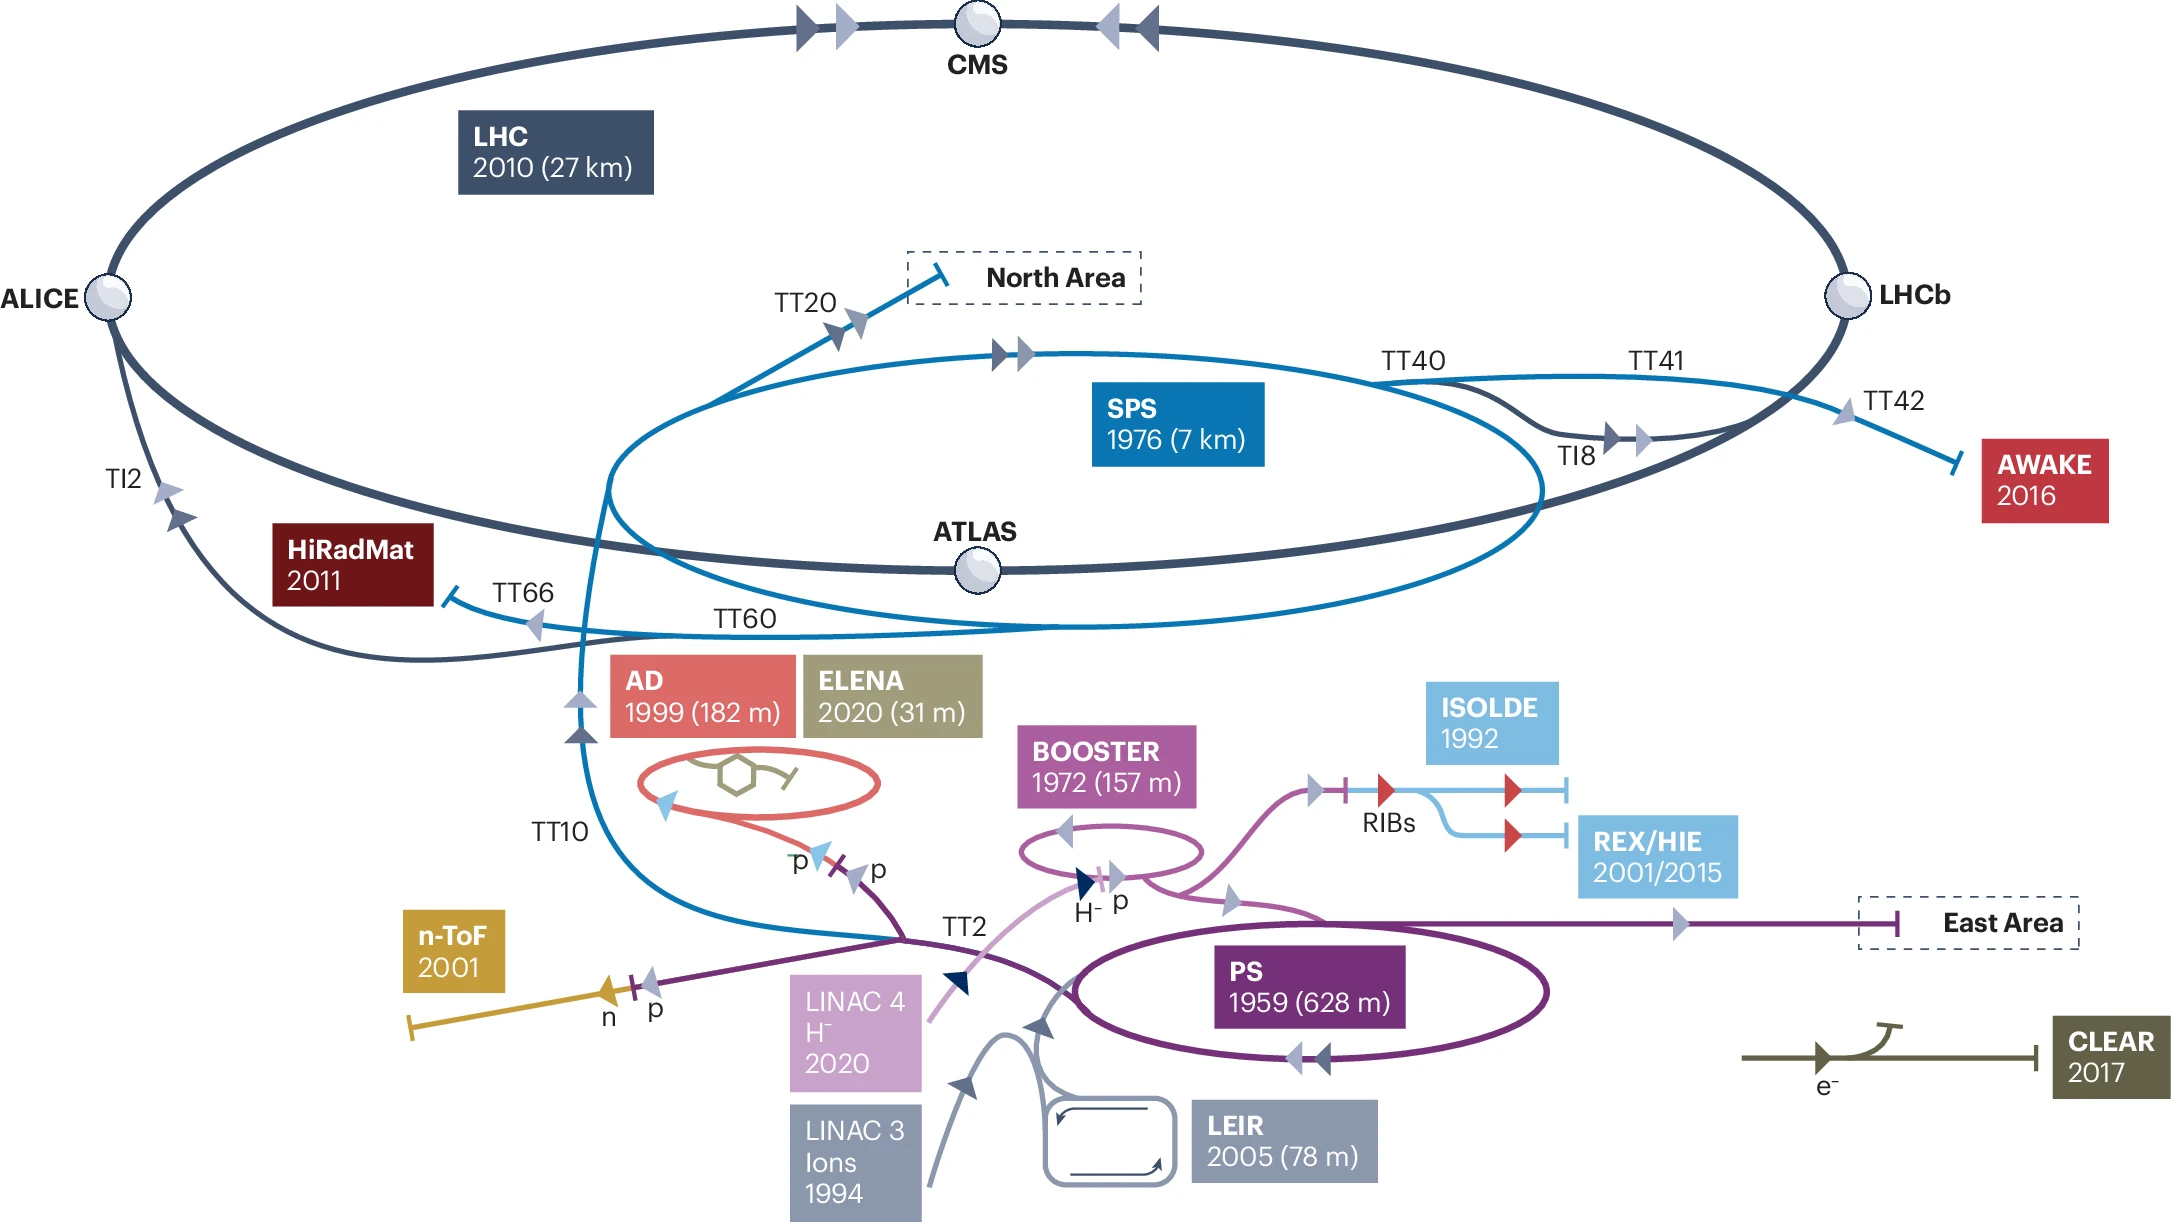
\includegraphics[width=1.0\textwidth]{images/CERN_Complex.png}
    \caption{Schematic overview of the CERN accelerator complex including main synchrotron accelerators LHC, SPS 
    and PS.}
    \label{fig:CERN_Complex}
\end{figure}

Achieving the desired collision energies requires the use of mutliple components of the CERN accelerator complex 
detailed in figure \ref{fig:CERN_Complex}, which consists of linear and smaller circular colliders - many of which were 
operated as independent experiments in the past. The acceleration is facilitated by an intricate setup of magnets (mostly 
dipoles and quadrupoles), which also steer and focus the beams. For proton-proton collisions this process starts with $H^-$ 
ions which are accelerated to $160\ MeV$ by a linear accelerator called Linac4. From there the ions are injected into the 
circular Proton Synchrotron Booster (PSB), which strips both electrons from the Hydrogen ions and creates a pure proton beam 
with an energy of $2\ GeV$. Afterwards the beam is accelerated to $26\ GeV$ by the Proton Synchrotron (PS) and $450\ GeV$ by 
the Super Proton Synchrotron (SPS) before finally being injected into the LHC where it is brought to its final collision 
energy. \par

%https://home.cern/news/news/accelerators/accelerator-report-excellent-2024-lhc-run-ended-abruptly
\begin{table}
\begin{center}
\caption{Overview of run periods of the LHC between 2008 and 2026.}
\label{table-lhc-runs}
\begin{tabular}{|c c c c|} 
 \hline
 Run Number & Years & Center of mass energy & Integrated Luminosity \\ [0.5ex] 
 \hline
 1 & 2008-2013 & $7-8\ TeV$ & $29.2\ fb^{-1}$ \\ 
 2 & 2015-2018 & $13\ TeV$ & $159.8\ fb^{-1}$ \\ 
 3 & 2022-2026 & $13.6\ TeV$ & $195.9\ fb^{-1}$ (up to and including 2024) \\ 
 \hline
\end{tabular}
\end{center}
\end{table}

The LHC has been operational since 2008, when it recorded its first proton-proton collisions at a center of mass energy 
of $7\ TeV$. Operation has been split into three distinct run periods denoted runs 1, 2 and 3 with shutdowns in between for 
maintenance and accelerator as well as detector upgrades. Details on the timeline of these runs, alongside achieved energy 
and luminosity is shown in table \ref{table-lhc-runs}. At present, run 1 is mostly relevant for historical reasons given the 
much lower center of mass energy and integrated luminosity. This research focuses on data collected during runs 2 and 3. These 
two run periods differ mainly by a slight increase in center of mass energy from $13$ TeV to $13.6$ TeV as well as an increase 
in the mean number of interactions per crossing from $<\mu> = 34$ to $<\mu> = 55$ as recorded by ATLAS and pictured in figure 
\ref{fig:Luminosity_vs_Pileup}. This difference results in a higher instantaneous luminosity for run 3, increasing total data 
volume as well as complexity of each recorded collision event due to excess pile-up.

%https://twiki.cern.ch/twiki/bin/view/AtlasPublic/LuminosityPublicResultsRun3
\begin{figure}
\centering
    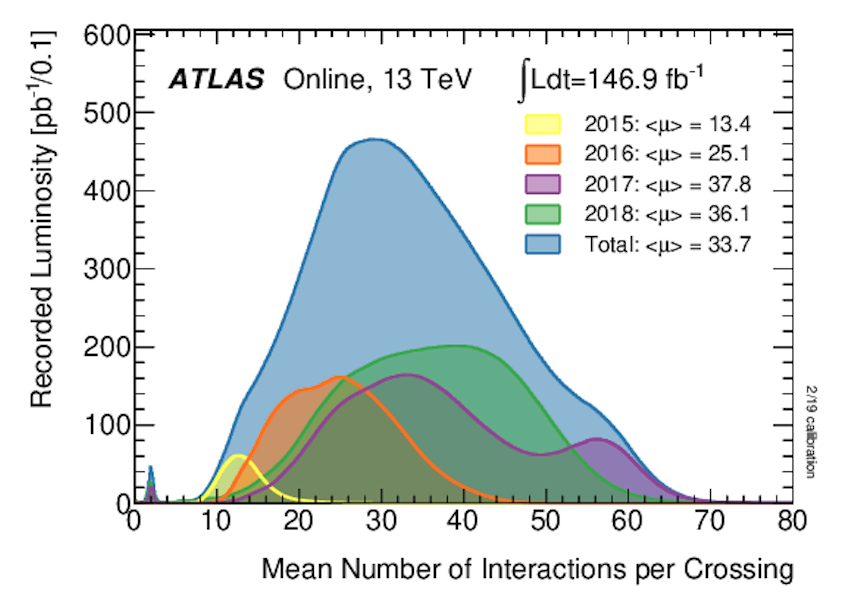
\includegraphics[width=0.6\textwidth]{images/Luminosity_vs_Pileup.png}
    \caption{Luminosity vs mean number of interactions for runs 1, 2 and 3 (up to September 17th 2025) as recorded by ATLAS.}
    \label{fig:Luminosity_vs_Pileup}
\end{figure}

\section{The ATLAS Detector}

ATLAS (\textbf{A} \textbf{T}oroidal \textbf{L}HC \textbf{A}pparatu\textbf{S}) is the largest of the four main detectors 
around the LHC ring. It is a general purpose detector designed to record the proton-proton collision signatures 
generated in the LHC without explicit focus on any specific process or particle type. This multi-purpose approach 
necessitates a highly modular detector with some trade-offs in detector design to balance cost and use. It is around 46 
meters long with a diameter of 25 meters and weights 7000 tons. The detector, visualized in its run 2 configuration in 
figure \ref{fig:ATLAS_Detector}, consists of four main active components: an inner tracking detector, two calorimeters 
and a muon spectrometer. \par

%https://cerncourier.com/a/atlas-undergoes-some-delicate-gymnastics/
\begin{figure}[h!]
\centering
    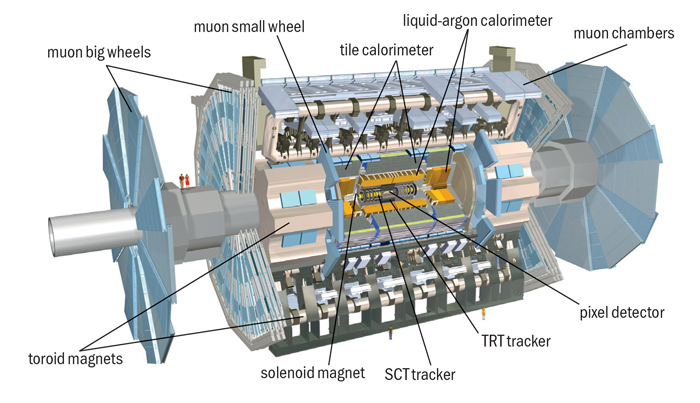
\includegraphics[width=0.8\textwidth]{images/ATLAS_Detector.jpg}
    \caption{Diagram showing all components of the ATLAS detector during run 2.}
    \label{fig:ATLAS_Detector}
\end{figure}

Each detector component interacts differently with different types of particles, as summarized in figure 
\ref{fig:Detector_Interactions}. The inner tracking detector located closest to the collision point and is primarily used for 
precise trajectory measurements of charged particles. The two components of the calorimeter system surround the inner detector 
and are mostly useful for energy measurements. An inner electromagnetic calorimeter mostly measures the energies of electrons 
and photons and an outer hadronic calorimeter measures the energies of charged and neutral hadrons. Finally, a muon spectrometer 
is located at the outside of the detector and is used to identify highly penetrating muons. Accurate measurements of particle 
momenta are possible because of a magnet system which curves the trajectories of charged particles traveling through the detector. 
A detailed overview of each detector component is presented in the following sections. While the overall configuration was kept 
relatively stable between runs 2 and 3, some changes were made in the so-called Phase-I upgrade which will be detailed where 
relevant \cite{atlas-run3-setup}. Furthermore, radiation damage results in the gradual degradation of the detector, inadvertently 
leading to slight differences in detector configuration over time.


%https://www.nbi.dk/~petersen/Teaching/Stat2011/Project1/project1.html
\begin{figure}
\centering
    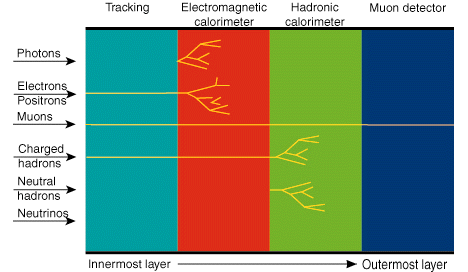
\includegraphics[width=0.8\textwidth]{images/Detector_Interactions.png}
    \caption{Sketch showing how different particles interact with detector components.}
    \label{fig:Detector_Interactions}
\end{figure}

\subsection{ATLAS Coordinate System}

An explanation of the details of the ATLAS detector requires an understanding the standardized coordinate system used in the 
experiment as well as some relevant physical quantities related to the particle trajectories. By convention, the coordinate 
system is centered at the collision point, with the beam line representing the z-axis, the x-axis pointing towards the center 
of the ring and the y-axis pointing towards the sky, as seen in figure \ref{fig:ATLAS_Coordinate_System}. The three important 
coordinates related to particle trajectories in this spherical coordinate system are the transverse momentum $p_T$, the 
azimuthal angle $\phi$ and the pseudorapidity $\eta$. The first of these is the projection of the momentum vector of a 
particle onto the transverse ($xy$) plane, which also defines the azimuthal angle measured starting from the positive x-axis. 
The final coordinate $\eta$ is a measure of the longitudinal component\footnote{This is frequently referred to as the "forward 
component"} of a particle trajectory and is related to the polar angle $\theta$ by $\eta = -ln(tan(\theta/2))$. By definition, 
$\eta = 0$ if the trajectory is entirely transverse and $\eta \rightarrow \infty$ as it approaches the beamline.

%https://tikz.net/axis3d_cms/
\begin{figure}
\centering
    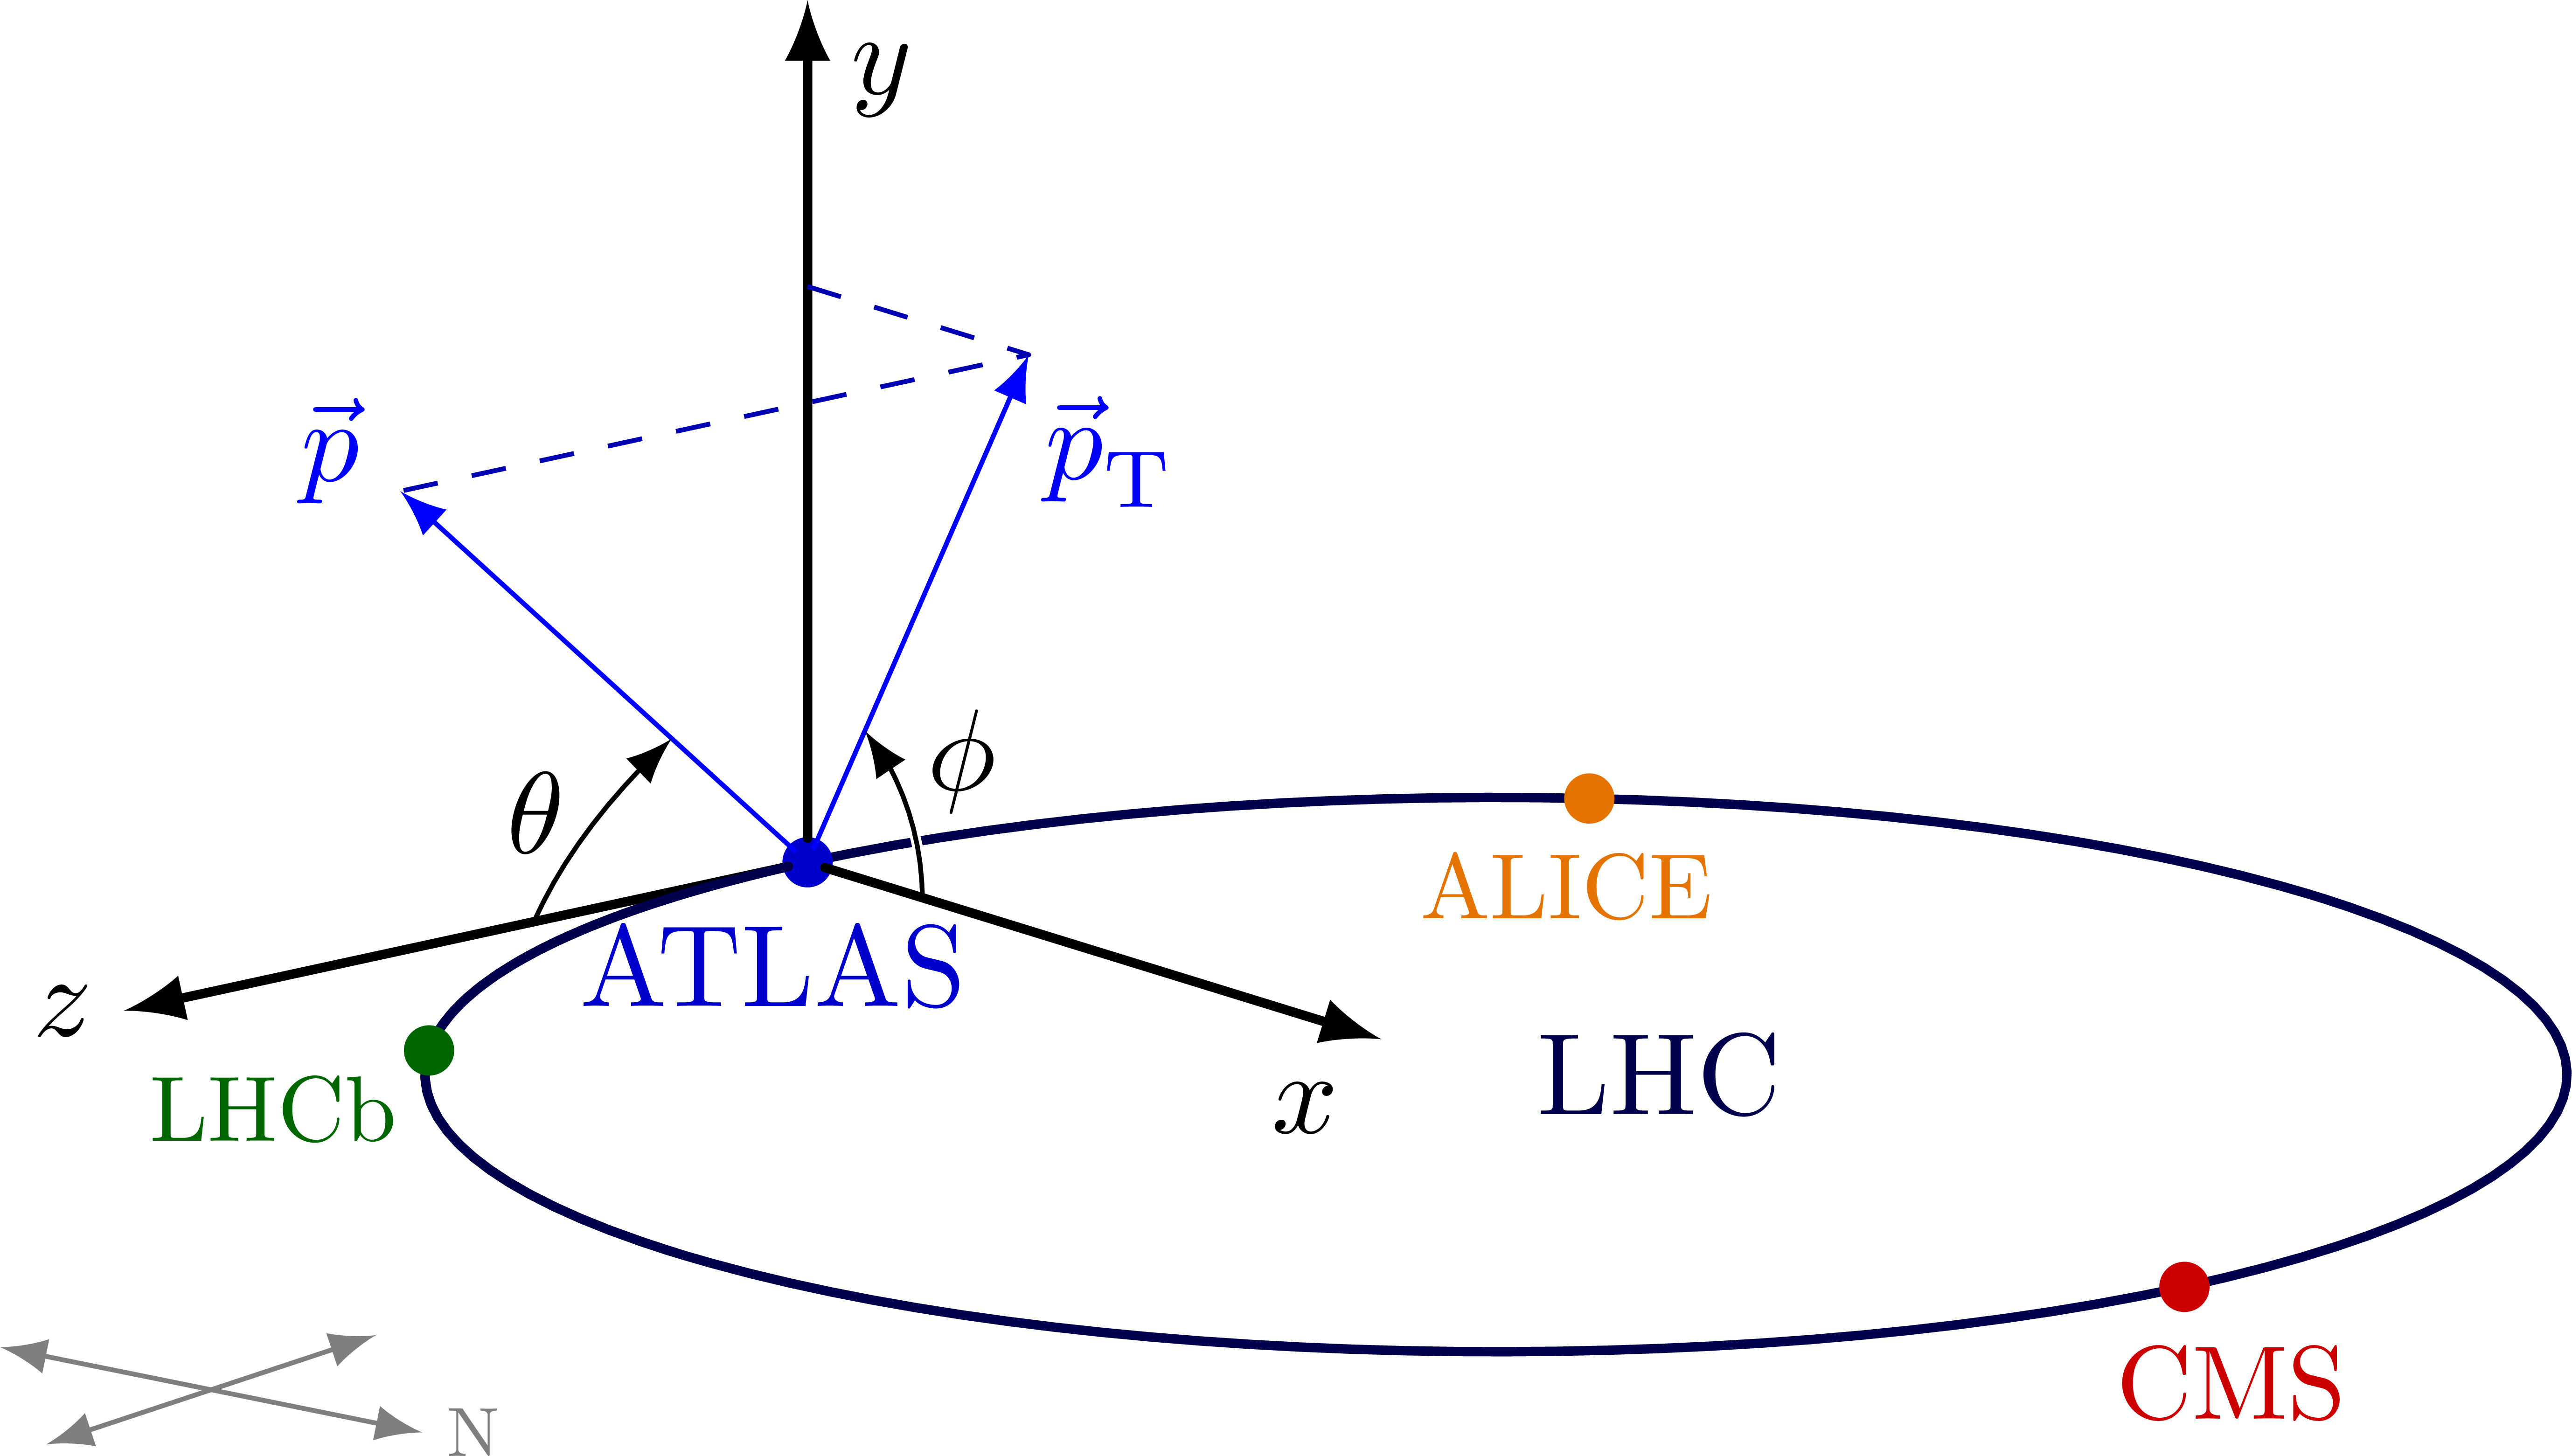
\includegraphics[width=0.6\textwidth]{images/ATLAS_Coordinate_System.png}
    \caption{Diagram showing the orientation of the coordinate system used in ATLAS as well as relevant kinematic 
    variables.}
    \label{fig:ATLAS_Coordinate_System}
\end{figure}

\subsection{Inner Tracking Detector}

The core of the ATLAS detector \cite{atlas-detector} is the inner tracking detector (ID), which is primarily responsible 
for precisely measuring the trajectories of charged particles by recording currents from electrons freed via the 
ionization of detector material. It is a combination of three different sub-systems: a pixel detector on the inside 
surrounded by a semiconductor tracker (SCT) and finally a transition radiation tracker (TRT) on the outside as shown in 
figure \ref{fig:ATLAS_Inner_Detector}. The pixel detector and SCT are built from silicon wafers while the TRT is made up 
of drift tubes filled with a Xenon-based gas mixture. Each subsequent part of the ID has larger elements and thus provides 
increasingly less granular position measurements. Geometrically the ID consists of barrel and endcap components where the 
barrel is a cylinder surrounding the beam and the endcaps are disks placed on either side of the barrel designed to detect 
forward particles with a total coverage of $|\eta| < 2.5$. \par

\begin{figure}
\centering
    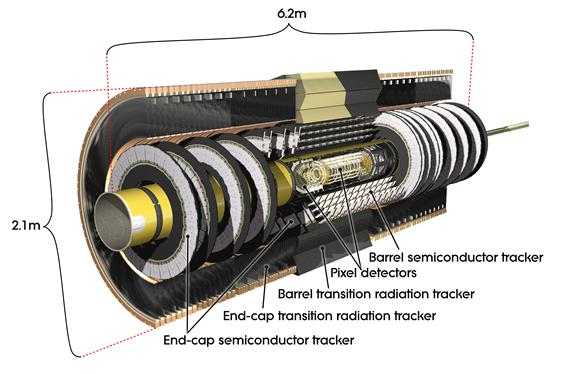
\includegraphics[width=0.8\textwidth]{images/ATLAS_Inner_Detector.png}
    \caption{Schematic of the ATLAS inner detector and its components for run 3 from \cite{atlas-run3-setup}.}
    \label{fig:ATLAS_Inner_Detector}
\end{figure}

The pixel detector \cite{pernegger-pixel-detector} is silicon-based and made up of 92 million individual sensor 
elements (pixels) arranged in 4 layers for the barrel component (1736 modules total) as well as 3 disk layers for each 
endcap (288 modules total). The innermost layer, called the insertable B-layer \cite{atlas-insertable-b-layer}, was 
inserted prior to run 2 of the LHC and is located a distance of $33mm$ from the beam pipe. It has the smallest individual 
pixel elements at $50\times250\ \mu m^2$, allowing for increased position resolution closest to the beam. The remaining 
layers have pixels of size $50\times400\ \mu m^2$, resulting in an overall spatial resolution of $\sim 8 \mu m$ in 
$r/\phi$ and $\sim 75 \mu m$ in $z$. All pixel sensors have a thickness of $250 \mu m$. Individual sensor elements 
are not arranged end to end but rather partially overlap to ensure complete $\phi$ coverage of each layer. The final 
layer of the pixel detector is located at $122.5mm$ from the beam. \par

Surrounding the pixel detector is the semiconductor tracker (SCT) \cite{atlas-sct}, which is similar in design and 
functionality, but contains larger silicon-based detector elements (strips). It is made up of 4 barrel layers (2112 
modules total) and 9 disk layers for each endcap (1976 modules total) starting at $299mm$ from the beam for the first 
barrel layer and ending at $514mm$ for the last. In total, the SCT contains over 6 million strips with a 
pitch\footnote{Pitch in this context refers to the distance between the center of adjacent detector elements} of 
$80\mu m$ and a length of $12cm$. To combat the low measurement resolution along the length of each strip, pairs of 
strips are rotated relative to each other on either side of a module. \par

The final sub-system of the ID is the transition radiation tracker (TRT) \cite{atlas-trt}, which differs quite 
significantly in design from the other two components. It consists of 300,000 gas filled drift tubes (or straws) with 
a thin wire at the center, each with a diameter of $4mm$. There are 50,000 straws of $144cm$ around the length of the 
barrel arranged parallel to the direction of the beam and extending outward to $1082mm$ from the beam line. A further 
250,000 straws of $39cm$ pointing outward radially from the beam are located in the two endcaps. In addition to 
ionization, charged particles passing through the TRT also emit transition radiation from crossing a boundary between 
two mediums with different dielectric constants. Since the amount of emitted radiation is inversely proportional to the 
mass of the particle crossing the boundary, the TRT can be used to discriminate between electrons and heavier charged 
particles such as pions. This gives it a unique advantage over the other ID sub-systems, although it comes at the cost 
of loss of measurement information along the longitudinal direction of the straws. \par

As mentioned before, the combination of these three sub-systems is mainly responsible for precise measurements of 
particle trajectories and momenta while minimally affecting their energies. This is accomplished by the presence of 
nearly 100,000,000 finely segmented individual readout channels spread across pixels, strips and straws. Overall, the 
inner detector achieves a momentum resolution of at least
\begin{equation}
\sigma_{pT}/p_T = 0.05\% p_T \oplus 1\%
\end{equation}
where $\oplus$ denotes an addition in quadrature. Resolution generally worsens with increased particle momentum due to 
the comparatively less pronounced curvature of high momentum tracks.

\subsection{Electromagnetic and Hadronic Calorimeters}

Surrounding the inner tracking detector of ATLAS is an extensive calorimeter system made up of both hadronic and 
electromagnetic sampling calorimeters. The purpose of these components is to stop incoming particles, making them 
deposit their energy to facilitate precise energy measurements as well as particle identification for photons, 
electrons and hadrons. To accomplish this, sampling calorimeter elements are made up of alternating layers of an 
absorbing material and an active material. The absorber is meant to be dense, triggering interactions with incoming 
particles which leads to particle showers\footnote{A particle shower is a cascade of particles produced in an 
interaction with detector material}. Electromagnetic showers proceed via repeated instances of Bremsstrahlung and 
$e^+e^-$ pair creation triggered by a single photon, electron or positron. Hadronic showers start with a break up of 
the incoming hadron (both charged and neutral), evolve into further interactions and usually also contain an 
electromagnetic component. Each section of active material then captures information about the energy of a shower 
via ionization or scintillation\footnote{These parts of the calorimeter are functionally identical to a tracking 
detector} from charged particle interactions. This process repeats through the layers of the calorimeter until all of 
the energy is deposited. The ATLAS calorimeter system uses two different technologies: a Liquid Argon (LAr) 
calorimeter on the inside and a Tile calorimeter on the outside. \par

\begin{figure}
\centering
    \includegraphics[width=0.8\textwidth]{images/ATLAS_Calorimeter.png}
    \caption{Schematic of the ATLAS calorimeters and their components for run 3 from \cite{atlas-run3-setup}.}
    \label{fig:ATLAS_Calorimeter}
\end{figure}

The inner LAr calorimeter system has both electromagnetic and hadronic components (as well as a separate forward 
calorimeter). Each of these uses Liquid Argon as the active material with different absorbers. The electromagnetic 
calorimeter covers all of the barrel as well as the interior section of the endcaps up to $|\eta| < 3.2$ and uses lead 
to stop photons and electrons up to a radiation length of $24X_0$\footnote{$X_0$ denotes the average length an electron 
needs to travel in material to reduce its energy by $1/e$}. The hadronic and forward components of the LAr calorimeter are 
restricted to the endcaps only and use copper and tungsten as absorbers respectively to capture forward hadrons up to 
$|\eta| < 4.9$. While hadrons lose part of their energy in the electromagnetic calorimeter, this is usually not enough 
to stop them completely. Because of this, the tile calorimeter, which is made out of steel and plastic scintillator, 
surrounds the LAr components in their entirety, providing a full hadronic calorimeter outside of the LAr endcaps. The 
energy resolution differs between these individual components as

\begin{equation} % EM calorimeter
(\sigma_{E}/E)_{EM} = 10\% / \sqrt{E} \oplus 0.7\%
\end{equation}

\begin{equation} % hadronic calorimeter for barrel and endcap, not forward
(\sigma_{E}/E)_{Had} = 50\% / \sqrt{E} \oplus 3\%
\end{equation}

\begin{equation} % hadronic calorimeter for forward
(\sigma_{E}/E)_{Fwd} = 100\% / \sqrt{E} \oplus 10\%
\end{equation}

\subsection{Muon Spectrometer}

The only remaining charged particles that reliably penetrate the electromagnetic and hadronic calorimeters are muons. 
Though inherently unstable, their relatively long lifetimes of $2.20\times10^{-6}\ s$ ensure they mostly don't decay 
within the detector at energies commonly seen in LHC collisions. They also generally do not interact significantly 
with detector material due to their much lower rates of energy loss via Bremsstrahlung, allowing them to keep 
comparatively undisturbed trajectories as they travel outward. As such, the outermost part of the ATLAS detector is a 
muon spectrometer (MS) used to identify muons and measure their momenta with coverage up to $|\eta| < 2.7$. Similar to 
the ID and calorimeter system, the MS also consists of a barrell and two endcaps. \par

The barrel is split into three concentric stations made up of Monitored Drift Tubes (MDT) as well as Resistive Plate 
Chambers (RPC) in the middle and outer station only. MDTs are tubes filled with a gas mixture which provide precision 
momentum measurements by measuring ionizing radiation (similar to the ID). There are 380,000 MDTs in the MS overall 
resulting in a momentum resolution of 

\begin{equation} % at pT = 1 TeV
\sigma_{pT}/p_T = 10\%
\end{equation}

RPCs use similar technologies but are optimized for speed rather than precision, allowing for quick muon identification. 
The endcaps of the MS are made up of 3 wheels each. Outer wheels contain MDTs only while the middle wheels contain both 
MDTs and Thin Gap Chambers (TGC), which are also optimized for speed. The inner (small) wheel was the subject of a major 
upgrade between runs 2 and 3 \cite{atlas-run3-setup}. In its run 2 configuration it consisted of MDTs, TGCs and Cathode 
Strip Chambers (CSC) which did not provide enough precision to deal with the increased number of interactions per event 
in run 3 conditions. To combat this they were entirely replaced by the New Small Wheels (NSW) which use Small-Strip Thin 
Gap Chambers (sTGC) and micro-mesh gaseous structure (Micromegas) detectors to achieve high speed muon identification 
with better momentum resolution than the run 2 wheels. \par

%https://link.springer.com/chapter/10.1007/978-3-030-52877-5_3
\begin{figure}
\centering
    \includegraphics[width=0.8\textwidth]{images/ATLAS_Muon_Spectrometer.png}
    \caption{Schematic of the ATLAS muon spectrometer for run 3 from \cite{atlas-run3-setup}.}
    \label{fig:ATLAS_Muon_Spectrometer}
\end{figure}

\subsection{Magnet System}

As previously discussed, making measurements of charged particle momenta relies on identifying the curvature of their 
trajectory in an applied magnetic field. Stronger fields provide more curved trajectories which improve momentum 
resolution, especially for high $p_T$ particles. In addition to the magnet system present in the LHC, which is 
responsible for the acceleration of the proton beams, the ATLAS detector has its own integrated magnet system 
(figure \ref{fig:ATLAS_Magnets}). The core of this is a solenoidal magnet around the ID, which applies a uniform $2T$ 
magnetic field along the direction of the beam. This means charged particles traveling from the collision point will 
follow helical trajectories with a pitch determined by their transverse momentum $p_T$ inside the ID. In addition to 
the interior solenoid there are three toroidal magnet systems made up of 8 coils each, one around the barrel portion 
of the detector and one around each of the end-caps. These provide a circular magnetic field up to $3.5T$ in the outer 
parts of the detector used to deflect the trajectories of muons for more accurate momentum measurements in the MS. \par

%https://link.springer.com/chapter/10.1007/978-3-030-52877-5_3
\begin{figure}
\centering
    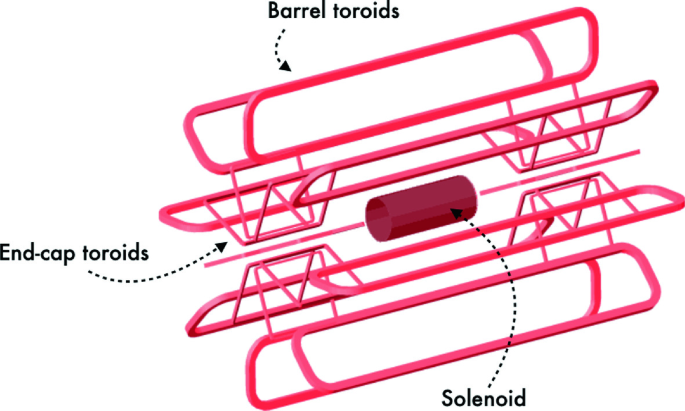
\includegraphics[width=0.6\textwidth]{images/ATLAS_Magnets.png}
    \caption{Schematic of the ATLAS magnet system.}
    \label{fig:ATLAS_Magnets}
\end{figure}

\subsection{Trigger and DAQ}

The LHC provided bunch crossing rate of up to 40 MHz floods the ATLAS detector with data in excess of what can 
realistically be recorded and stored. Much of this data comes from collision events likely to contain little of 
interest to a physicist on the ATLAS experiment\footnote{For example, events where no "hard scatter" collision 
takes place (i.e. pile-up events)}. To combat this, decisions need to be made about whether individual events are 
worth recording and storing, which is the responsibility of the ATLAS Trigger and Data Acquisition (DAQ) systems. The 
combined effect of all experimental triggers reduces the frequency of recorded events from 40 MHz to around 3 kHz 
for both run 2 and 3 \cite{oliveiradamazio-trigger}. This is accomplished with two sequentially applied systems: the 
Level-1 Trigger (L1) and the High Level Trigger (HLT). \par

\begin{figure}
\centering
    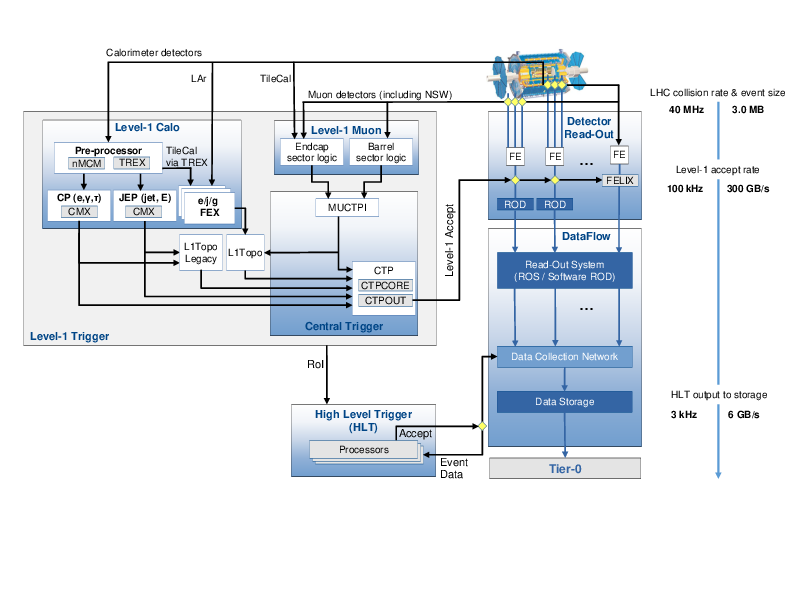
\includegraphics[width=1.0\textwidth]{images/Trigger_System.png}
    \caption{Diagram showing the core components of the ATLAS Trigger and DAQ for run 3 from \cite{atlas-run3-setup}.}
    \label{fig:Trigger_System}
\end{figure}

The L1 trigger is a hardware trigger that filters events by identifying large energy deposits in the calorimeter 
(L1-Calo) as well as high $p_T$ muons in the fast-response muon system (L1-Muon). For run 3, the granularity of 
calorimeter information passed to L1-Calo was increased significantly to account for the expected increase in 
energy deposits from additional pile-up. L1-Muon was also augmented through an increase in the number of modules 
factored in as well as the replacement of the small wheel \cite{atlas-run3-trigger}. The Central Trigger Processor 
(CTP) records events based on both individual hardware triggers as well as their combination via computation of the 
pairwise invariant masses of muons and energy clusters in the calorimeter (L1-Topo). Events passing L1 undergo a 
lightweight version of the object reconstruction chain (described in detail in the next section) and get passed 
through the HLT, where a set of more complex criteria are applied to reduce the number of events further while 
covering a large number of different physics interests.

\section{Object Reconstruction}

The procedure of turning raw detector measurements into objects with physically interpretable characteristics is 
called object reconstruction. It represents the first step in going from a series of abstract energy deposits in 
the ATLAS detector to a measurement of the $H \rightarrow c\bar{c}$ process. The core of this is the reconstruction 
of particle trajectories, which combines individual measurements in segments of the inner detector into tracks with 
associated momenta. Energy deposits in the calorimeter are also clustered and matched with to tracks in an attempt 
to separate contributions from neutral and charged particles. With this fundamental information, certain particles 
(such as electrons, photons and muons) can be directly identified and particle jets created by the hadronization of 
quarks can be reconstructed. Development of these reconstruction algorithms relies on Monte Carlo (MC) simulated 
events, requiring careful checks to ensure parity in performance between MC and data via a procedure called 
calibration. This chapter outlines all aspects of the object reconstruction chain to give a complete picture of the 
low level physics objects relevant to measurements of physical processes in the ATLAS detector. \par

\subsection{Fundamental Objects: Tracks, Clusters and Vertices}

The first step in the ATLAS reconstruction chain is identifying trajectories of particles passing through the 
inner detector \cite{cornelissen-tracking}. Specifically we are interested in reconstructing a set of parameters 
given by $(d_0, z_0, \phi, \theta, \frac{q}{p})$ shown in figure \ref{fig:Impact_Parameters} from individual energy 
deposits ("hits") in the detector. The transverse and longitudinal impact parameters (IP) $d_0$ and $z_0$ are 
defined to be the coordinates of the point of closest approach between a track and the primary interaction point 
when the track is fully extrapolated in both directions. This functions as a measure of whether a track is likely 
to have originated from the primary interaction point (small IP) or from some later decay or interaction or pile-up 
(large IP). The other 3 tracking variables are previously discussed representations of the particle 4-vector. \par

%https://indico.nbi.ku.dk/event/758/attachments/1684/2344/trackingnote.pdf
\begin{figure}
\centering
    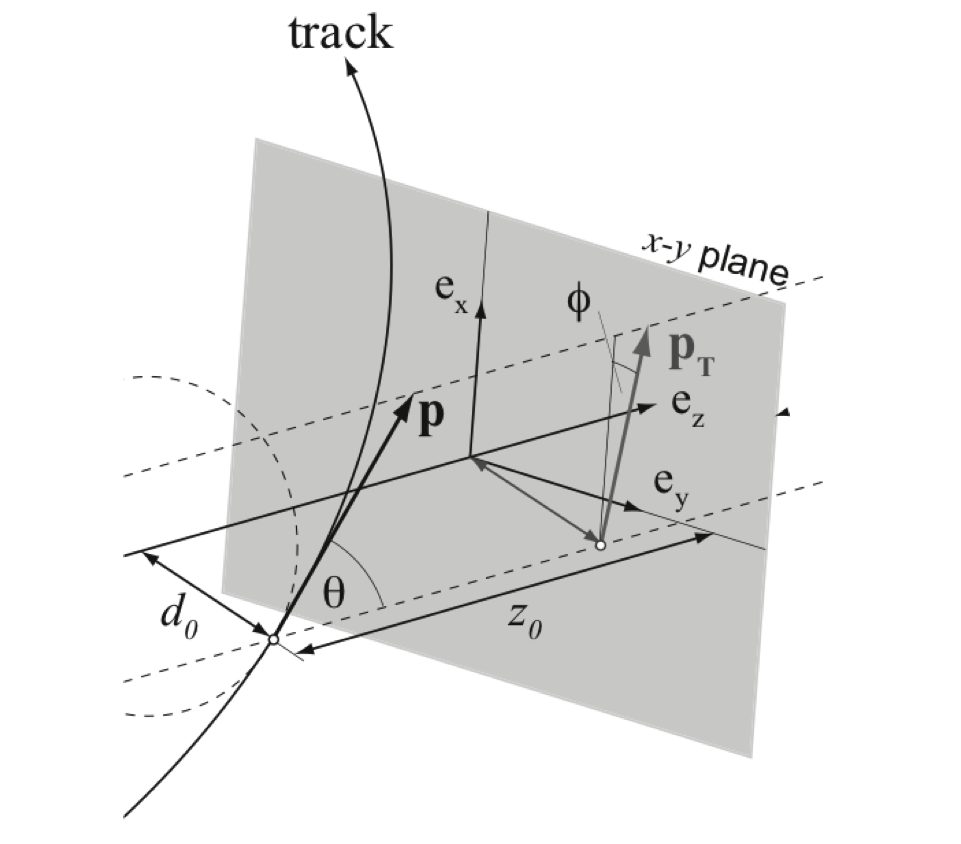
\includegraphics[width=0.8\textwidth]{images/Impact_Parameters.png}
    \caption{Diagram visualizing track parameters used in ATLAS.}
    \label{fig:Impact_Parameters}
\end{figure}

Tracking begins with a process called spacepoint formation, which clusters adjacent hits reaching some energy 
threshold in each layer of the pixel and SCT detectors. These clusters are transformed into global coordinates 
representing individual intersection points between particle trajectories and detector material. Spacepoints in 
subsequent layers are then grouped into batches of 3 to create track seeds. This is preferentially done in the SCT 
due to the lower density of spacepoints, but pixel seeds are also considered. Each seed is required to meet specific 
quality criteria based on rough estimates of track paramters to minimize the presence of duplicate seeds for a given 
track and reduce computational overhead. The remaining seeds are then extended in both directions via a track 
finding algorithm based on the combinatorial Kalman filter (CKF) \cite{fruehwirt-kalman-filter}. This algorithm 
repeatedly adds compatible clusters on adjacent layers to a track candidate and smoothes the estimated trajectory 
taking into account detector resolution effects. In the case where multiple compatible spacepoints are found, 
diverging track candidates are created and extended separately. Additionally, a prodedure called Bremsstrahlung 
recovery allows seeds that fail the track finding step entirely to be considered with a decreased quality threshold. 
This procedure is triggered when a failed seed is matched to an interesting region in the calorimeter, which helps 
recover performance for electron tracks radiating photons through Bremsstrahlung as they traverse the detector. \par

Once the full set of track candidates is established via the CKF, an ambiguity resolution stage attempts to remove 
all fake and duplicate tracks by enforcing a more stringent set of quality criteria. Tracks with a significant 
amount of overlapping (shared) hits are compared against each other and only the highest quality track is retained. 
However, due to the dense tracking environment of ATLAS (particularly in the pixel detector), a limited number of 
shared hits between tracks is allowed. A dedicated algorithm is used to perform cluster splitting 
\cite{atlas-cluster-splitting}, which aims to split clusters consisting of multiple particles into their individual 
components. After ambiguity resolution, a $\chi^2$ fit is performed on the remaining candidates for a final track 
parameter estimate. Where applicable, an attempt is made to extend track candidates made from pixel and SCT hits 
into the TRT via another Kalman filter based algorithm. These extensions are only retained if the overall $\chi^2$ 
fit of a track does not worsen with the additional TRT hits. Aside from this forward tracking procedure, a 
secondary back-tracking pass is done to increase reconstruction efficiency of particles produced further from the 
beam. This procedure is mostly identical to forward tracking, but starts by searching for hit segments in the TRT 
aligned with regions containing significant energy deposits in the calorimeter. Seeds are then created in layers 
of the pixel and SCT detectors consistent with these TRT segments using two spacepoints only. While the overall 
approach to tracking is very similar between the run 2 and run 3 reconstruction chain, various speed ups and other
improvements were introduced to deal with the denser tracking environment from increased pile-up under run 3 
conditions \cite{atlas-run3-tracking}. This includes changes to seed and track quality requirements at multiple 
steps of the chain as well as earlier stopping for bad candidates, allowing for the retention of a fast, high 
efficiency track reconstruction chain. \par 

Separately, energy deposits in the calorimeter are grouped into so called topo-clusters using a dedicated clustering 
algorithm \cite{atlas-calo-cluster} and then split to reflect the presence of multiple particle contributions where 
applicable. In particular, this happens when deposits are topologically close to each other but contain multiple 
separable energy peaks. For many practical applications tracks and calorimeter clusters are matched to each other via 
an algorithm called "Particle Flow" (PFlow) \cite{atlas-pflow}. PFlow is also used to estimate the energy contribution 
of a charged particle track to a topo-cluster allowing for the isolation of neutral contributions and treatment as 
separate objects. This results in a unified description of neutral and charged particles measured in the detector 
via a combination of information from tracks and topo-clusters. \par

The presence of pile-up interactions leads to the reconstruction of excess tracks and calorimeter clusters that are not 
relevant to the interaction of interest identified by the trigger system. To mitigate the impact of these additional 
objects in selections enforced by physics analyses, a primary event vertex corresponding to the location of the hard 
scatter collision is identified via a vertex finding and fitting algorithm that differs slightly between run 2 and run 3 
\cite{atlas-vertex-reco-run2, atlas-vertex-reco-run3}. In run 2, the process begins by creating an initial vertex seed 
centered at the beam-spot in the transverse plane and the mode of the z-position of all tracks passing some basic 
kinematic cuts. All tracks within a certain impact parameter window of this seed are then considered in a Kalman filter 
based fit that iteratively associates nearby tracks and recomputes the vertex position based on $\chi^2$ compatibility. 
Once this minimization converges, all tracks with a sufficient compatibility to the final vertex position are removed 
from the pool and the process is repeated. The run 3 version of the algorithm uses a Gaussian density function for 
seeding and allows each track to be associated with multiple vertices in the fit via a calculated weight. After multiple 
iterations of the fit, each track ends up primarily associated with a single vertex only. In both cases after fit 
convergence the vertex with the largest $\Sigma p_T^2$ is marked as the primary vertex. The position of this primary 
vertex can be used to remove tracks that likely originate from pile-up interactions based on their impact parameters. 
\par

\subsection{Electrons and Photons}

Electrons ($e^{\pm}$) and photons ($\gamma$) are some of the most easily identifiable fundamental particles 
observable in the ATLAS detector due to their unique interaction signatures in the EM calorimeter. A dedicated 
$e^{\pm}/\gamma$ reconstruction chain, which is built on top of track and calorimeter cluster reconstruction, exists to 
find and isolate these signatures \cite{atlas-electrons-photons-reco}. This chain begins by considering topo-clusters 
above a minimum energy threshold ($400\ MeV$ in run 2) and with more than 50\% of their energy deposited in the EM 
calorimeter. Clusters that pass these criteria provide the basis of both electron and photon reconstruction, which 
proceed somewhat independently. Electrons leave tracks in the ID while photons only do so if they undergo 
$\gamma \rightarrow e^+e^-$ conversion before they enter the calorimeter. As such, different track to cluster matching 
procedures exist to cover these three cases. \par

Clusters matched to at least one standard particle track in the ID with $|\Delta\eta| < 0.05$ and 
$-0.10 < q*(\phi_{track}-\phi_{cluster}) < 0.05$ are considered electron candidates. If multiple tracks fulfill these 
criteria, tracks with hits in the pixel detector and a better $\Delta R$ match to the cluster are preferred. Converted 
photon candidates are identified by matching clusters to conversion vertices, which are built by considering either 
two tracks with opposite charges or single tracks without hits in the innermost detector layers. In either case, 
relevant tracks must have signatures in the TRT consistent with electrons and vertex candidates must likely be from 
a massless particle. In case of multiple matches, two track vertices with hits in the Silicon detectors (pixel or SCT) 
are preferred. Remaining unmatched topo-clusters are considered unconverted photon candidates. \par

To account for radiation from Bremsstrahlung, a separate cluster matching procedure is performed for all electron and 
photon candidates, grouping individual topo-clusters into superclusters. Starting from the cluster with the highest 
transverse energy $E_T$, electron seed clusters are required to have $E_T > 1\ GeV$ and be matched to a track with 
at least 4 hits in the Silicon detectors. Photon seed clusters have no vertex matching requirement, but must have 
$E_T > 1.5\ GeV$. Surrounding (satellite) clusters are then associated to the seed cluster if they are within a window 
of $\Delta\eta\times\Delta\phi =0.075\times0.125$, which is extended to $\Delta\eta\times\Delta\phi =0.125\times0.300$ 
for electrons in cases where the best matched track of the seed cluster is also the best match for the satellite 
cluster. For converted photons, clusters where the best matched track belongs to the matched conversion vertex of the 
seed cluster are also added. Once the superclusters are built, relevant variables related to energy and shower shape 
are recomputed and the track and conversion vertex matching procedure is repeated. \par

In order to improve the purity of reconstructed electron and photon objects, a selection procedure is applied to all 
candidates. For electrons, this is intended to distinguish prompt electrons from hadronic objects, converted photons 
and electrons originating from secondary decays. A likelihood discriminant based on variables describing the properties 
of the electron track, the associated calorimeter clusters and their compatibility is built for each candidate. This 
discriminant is used to define a series of cuts or "working points" (WP) based on electron reconstruction efficiency 
in MC simulations. They are referred to as loose, medium and tight where tight provides the highest signal purity and 
lowest background contamination. For photons the loose, medium and tight WPs are defined based on direct cuts on 
individual variables rather than a combined discriminant in an otherwise similar procedure. These are intended to 
separate prompt photons from hadronic backgrounds. \par

In addition to selection requirements, all electrons and photons have two associated isolation variables which allow 
individual analysis groups in ATLAS to apply cuts based on spatial isolation of electrons or photons in the calorimeter 
and ID. Calorimeter isolation is defined as the sum of $E_T$ of topo-clusters around the electron or photon cluster 
after subtracting an estimated contribution from pile-up. Similarly, the track isolation is defined to be the sum of 
$p_T$ of tracks within a cone of the electron track or photon cluster direction. Separate loose and tight electron and 
photon isolation WPs are derived based on these two variables in MC simulations in a similar fashion to the isolation 
WPs. \par

In order to ensure parity between selection and isolation efficiency WPs in data and MC simulation, the impact of all WP 
based cuts are compared between the two. In particular, scale factors representing the ratio of data efficiency to MC 
efficiency are derived in bins of photon/electron $E_T$ and $\eta$ for each WP. For electrons this is done by selecting 
$Z \rightarrow e^+e^-$ and $J/\Psi \rightarrow e^+e^-$ events, resulting in scale factors deviating from unity by less 
than 5-7\% for all bins across both selection and isolation WPs \cite{atlas-electrons-photons-eff}. Corresponding 
uncertainties are generally less than 1\% for identification and up to 5\% for isolation. For photons, scale factors and 
corresponding uncertainties are derived in $Z \rightarrow e^+e^-\gamma$ events and are similarly within 5\% of unity with 
uncertainties of up to 7\%. \par

\subsection{Muons}

Muons ($\mu^{\pm}$) are easily identifiable by their detector signatures for very different reasons than their lighter 
$e^{\pm}$ counterparts. Due to their long lifetimes and much lower rates of energy loss via Bremsstrahlung they penetrate 
far into the detector and commonly leave traces in all subsystems\footnote{Muons are essentially treated as minimum-ionizing 
particles}. While tracks in the muon system are the most obvious sign for their presence, muon reconstruction takes 
signatures across all parts of the detector into account. To this end there are five different algorithms focusing on 
different subsystem combinations to identify five types of muons: combined (CB), inside-out combined (IO), muon-spectrometer 
extrapolated (ME), calorimeter-tagged (CT) and segment-tagged (ST) \cite{atlas-muons}. In general, muon reconstruction starts 
with the search for continuous track segments in each sector of the MS. This differs from standard track reconstruction due 
to the sparser tracking environment and is done via Hough transform on the individual detector hits for every sector 
\cite{illingworth-hough-transform}. Reconstructed track segments are then matched across sectors based on their estimated 
IPs and parabolic trajectories which estimate the path of a muon in the applied magnetic field. Finally, a $\chi^2$ fit is 
performed to build track candidates which is used as a basis to remove outlier hits and add unmatched hits along the fitted 
trajectory. Ambiguity resolution ensures that only the highest quality track is retained when there is significant hit 
overlap. \par

CB muons are reconstructed by matching tracks in the ID and the MS while factoring in energy loss in the calorimeter and 
performing a combined fit. At $|\eta| > 2.5$ the requirements are loosened to allow for shorter track segments in the Silicon 
detectors to be matched to tracks in the MS. IO muon reconstruction uses the same information, but performs inside-out 
association by starting from ID tracks and searching for at least 3 associated hits in the MS rather than a fully reconstructed 
muon track segment. When an ID track satisfies tight angular matching with at least one muon track segment it is classified as 
an ST muon and adopts its parameters directly from the track fit in the ID. Remaining tracks in the muon system are considered 
ME muons and are extrapolated back to the interaction point directly without further matching. CT muons do not rely on 
information from the MS at all but are rather reconstructed by extrapolating tracks from the ID to the calorimeter and checking 
for signatures consistent with minimum-ionizing particles. For these, track parameters are also adopted directly from the ID fit. 
For each reconstruction method a minimum muon $p_T$ cut of 2 GeV is applied, except for a raised threshold of 5 GeV for CT muons 
given the larger amount of backgrounds that are otherwise vetoed by matched MS signatures. \par

After all muon candidates are reconstructed, various selection criteria are applied based on the number of hits in ID subsystems 
and MS sectors for each track, the compatibility of the track segments and overall fit properties. As with photons and electrons, 
a set of loose, medium and tight selection WPs are defined based on these criteria. These WPs are identified based on their prompt 
muon reconstruction efficiency and hadron misidentification rate, allowing individual analyses to balance the two as needed. There 
are also separate WPs defined for high-$p_T$ and low-$p_T$ muon identification to cover more specific use cases. In order to 
reject non-prompt muons originating from secondary decays of hadrons, a cut on the transverse and longitudinal impact parameters 
is enforced as $|d_0|/\sigma(d_0) < 3$ and $|z_0|\text{sin}\theta < 0.5$ mm. \par

Further isolation of prompt muons is enforced via two isolation variables: track-based isolation and calorimeter-based isolation. 
This serves mainly to further reduce the number of reconstructed muons originating from hadron decays and mirrors the approach 
taken for photons and electrons. In particular, track-based isolation is calculated by summing the $p_T$ of all tracks within a 
cone of a particular size around a muon track. Calorimeter-based isolation is defined to be the sum of $E_T$ deposited in the 
calorimeter within a cone of the extrapolated muon track while removing the expected muon contribution. A series of isolation WPs 
are defined based on either track-isolation only or a combination of both variables, using different cone sizes and cuts to 
optimize prompt muon retention and non-prompt muon rejection. \par

Finally, a calibration procedure is applied to understand the differences in muon reconstruction efficiency across data and MC 
simulations using $Z \rightarrow \mu^+\mu^-$ and $J/\Psi \rightarrow \mu^+\mu^-$ events. SFs are derived for all selection WPs 
in bins of $(\eta, \phi)$ and in $(p_T, \eta)$ for isolation WPs. They are generally close to unity with uncertainties of up to 
a few percent depending on the WP and bin. \par

\subsection{Particle Jets}

\subsection{Hadronic Taus and Missing Energy}